\documentclass[../capitulos/cap1.tex]{subfiles}

\tikzset{every picture/.style={line width=0.75pt}} %set default line width to 0.75pt        

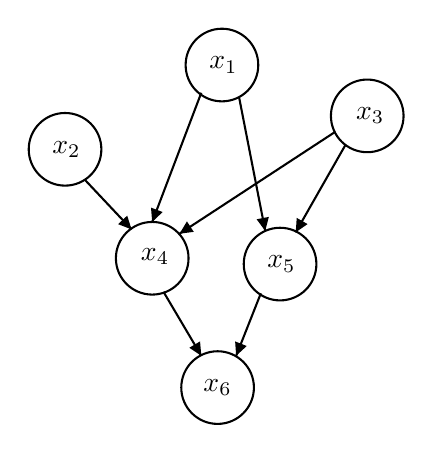
\begin{tikzpicture}[x=0.75pt,y=0.75pt,yscale= -0.7,xscale= 0.7]
%uncomment if require: \path (0,300); %set diagram left start at 0, and has height of 300

\draw    (332, 42) circle [x radius= 25, y radius= 25]  ;
\draw    (224, 100) circle [x radius= 25, y radius= 25]  ;
\draw    (432, 77) circle [x radius= 25, y radius= 25]  ;
\draw    (284, 175) circle [x radius= 25, y radius= 25]  ;
\draw    (372, 179) circle [x radius= 25, y radius= 25]  ;
\draw    (329, 264) circle [x radius= 25, y radius= 25]  ;
\draw    (343.78,64.11) -- (361.78,156.11) ;
\draw [shift={(361.78,156.11)}, rotate = 258.93] [fill={rgb, 255:red, 0; green, 0; blue, 0 }  ] [draw opacity=0] (8.93,-4.29) -- (0,0) -- (8.93,4.29) -- (8.93,-4.29)    ;

\draw    (317.78,61.11) -- (284,150) ;
\draw [shift={(284,150)}, rotate = 290.81] [fill={rgb, 255:red, 0; green, 0; blue, 0 }  ] [draw opacity=0] (8.93,-4.29) -- (0,0) -- (8.93,4.29) -- (8.93,-4.29)    ;

\draw    (237.78,121.11) -- (269.78,155.11) ;
\draw [shift={(269.78,155.11)}, rotate = 226.74] [fill={rgb, 255:red, 0; green, 0; blue, 0 }  ] [draw opacity=0] (8.93,-4.29) -- (0,0) -- (8.93,4.29) -- (8.93,-4.29)    ;

\draw    (417,97) -- (382.78,157.11) ;
\draw [shift={(382.78,157.11)}, rotate = 299.65] [fill={rgb, 255:red, 0; green, 0; blue, 0 }  ] [draw opacity=0] (8.93,-4.29) -- (0,0) -- (8.93,4.29) -- (8.93,-4.29)    ;

\draw    (409.78,88.11) -- (302.78,158.11) ;
\draw [shift={(302.78,158.11)}, rotate = 326.81] [fill={rgb, 255:red, 0; green, 0; blue, 0 }  ] [draw opacity=0] (8.93,-4.29) -- (0,0) -- (8.93,4.29) -- (8.93,-4.29)    ;

\draw    (291.78,198.11) -- (317.78,242.11) ;
\draw [shift={(317.78,242.11)}, rotate = 239.42000000000002] [fill={rgb, 255:red, 0; green, 0; blue, 0 }  ] [draw opacity=0] (8.93,-4.29) -- (0,0) -- (8.93,4.29) -- (8.93,-4.29)    ;

\draw    (358.78,199.11) -- (341.78,242.11) ;
\draw [shift={(341.78,242.11)}, rotate = 291.57] [fill={rgb, 255:red, 0; green, 0; blue, 0 }  ] [draw opacity=0] (8.93,-4.29) -- (0,0) -- (8.93,4.29) -- (8.93,-4.29)    ;


\draw (333,42) node   {$x_{1}$};
\draw (225,100) node   {$x_{2}$};
\draw (434,77) node   {$x_{3}$};
\draw (286,174) node   {$x_{4}$};
\draw (373,179) node   {$x_{5}$};
\draw (329,264) node   {$x_{6}$};


\end{tikzpicture}